\section{Surveyed Discoveries}

Survey data is available for the entire Tolminski Migovec plateau on the Imperial College Caving Club website in Survex format.\\

An alphabetically sorted list of new discoveries during Vodna Sled 2010 is presented here:\\

\begin{tabular}{l c}
Name & Polygon Length \\
\midrule
Black Knight & 116.08 m \\
Consort & 239.99 m \\
Crack in Time & 44.60 m \\
Esoterica & 63.24 m \\
Insomnia & 100.30 m \\
It Will Rain & 48.92 m \\
Kamikaze & 159.60 m \\
Korita & 86.39 m \\
Lost Hopes & 35.62 m \\
Palace of King Minos & 589.63 m \\
Mudstone & 53.36 m \\
Povodni Moz2 & 161.20 m \\
Povodni Moz & 27.69 m \\
Rolling & 48.27 m \\
Serpentine & 70.53 m \\
Sidewinder & 23.86 m \\
Stalemate & 35.73 m \\
Surprise & 71.24 m \\
White Bishop & 52.86 m \\
Wonderland & 134.29 m \\
\midrule
Total & 2163.40 m \\
\end{tabular}

\subsection{Vrtnarija Loop Closures}

Our survey is now corrected to grid north based on the NOAA American
Webservice, with Lat + Long on M10/Bivi, calculated for 1st Aug of each year.
This was mainly to agree with surface DEM data \& GPS data (declination is
approximately 2.5 degrees), as the rate of change of declination is slow (6
minutes a year).

\passage{Vrtnarija} possess two large loops, making the cave into a `figure 8' configuration. 

During 2009 the \passage{Captain Kangaroo} --- main pitch series loop was closed
(consisting of data collected from 2000--2009, approximately 1.8km loop).
During 2010 the \passage{Tolminska Korita} -- \passage{Big Rock} loop was closed (data from
2001--2010, approximately 1.7km loop).

All sampled misclosures were 1.5--2.0 \%. Typically the horizontal misclosure
was twice that of the vertical (our total plan length of survey polygon is also
approximately double the total vertical length).




\begin{pagesurvey}
\centering
\frame{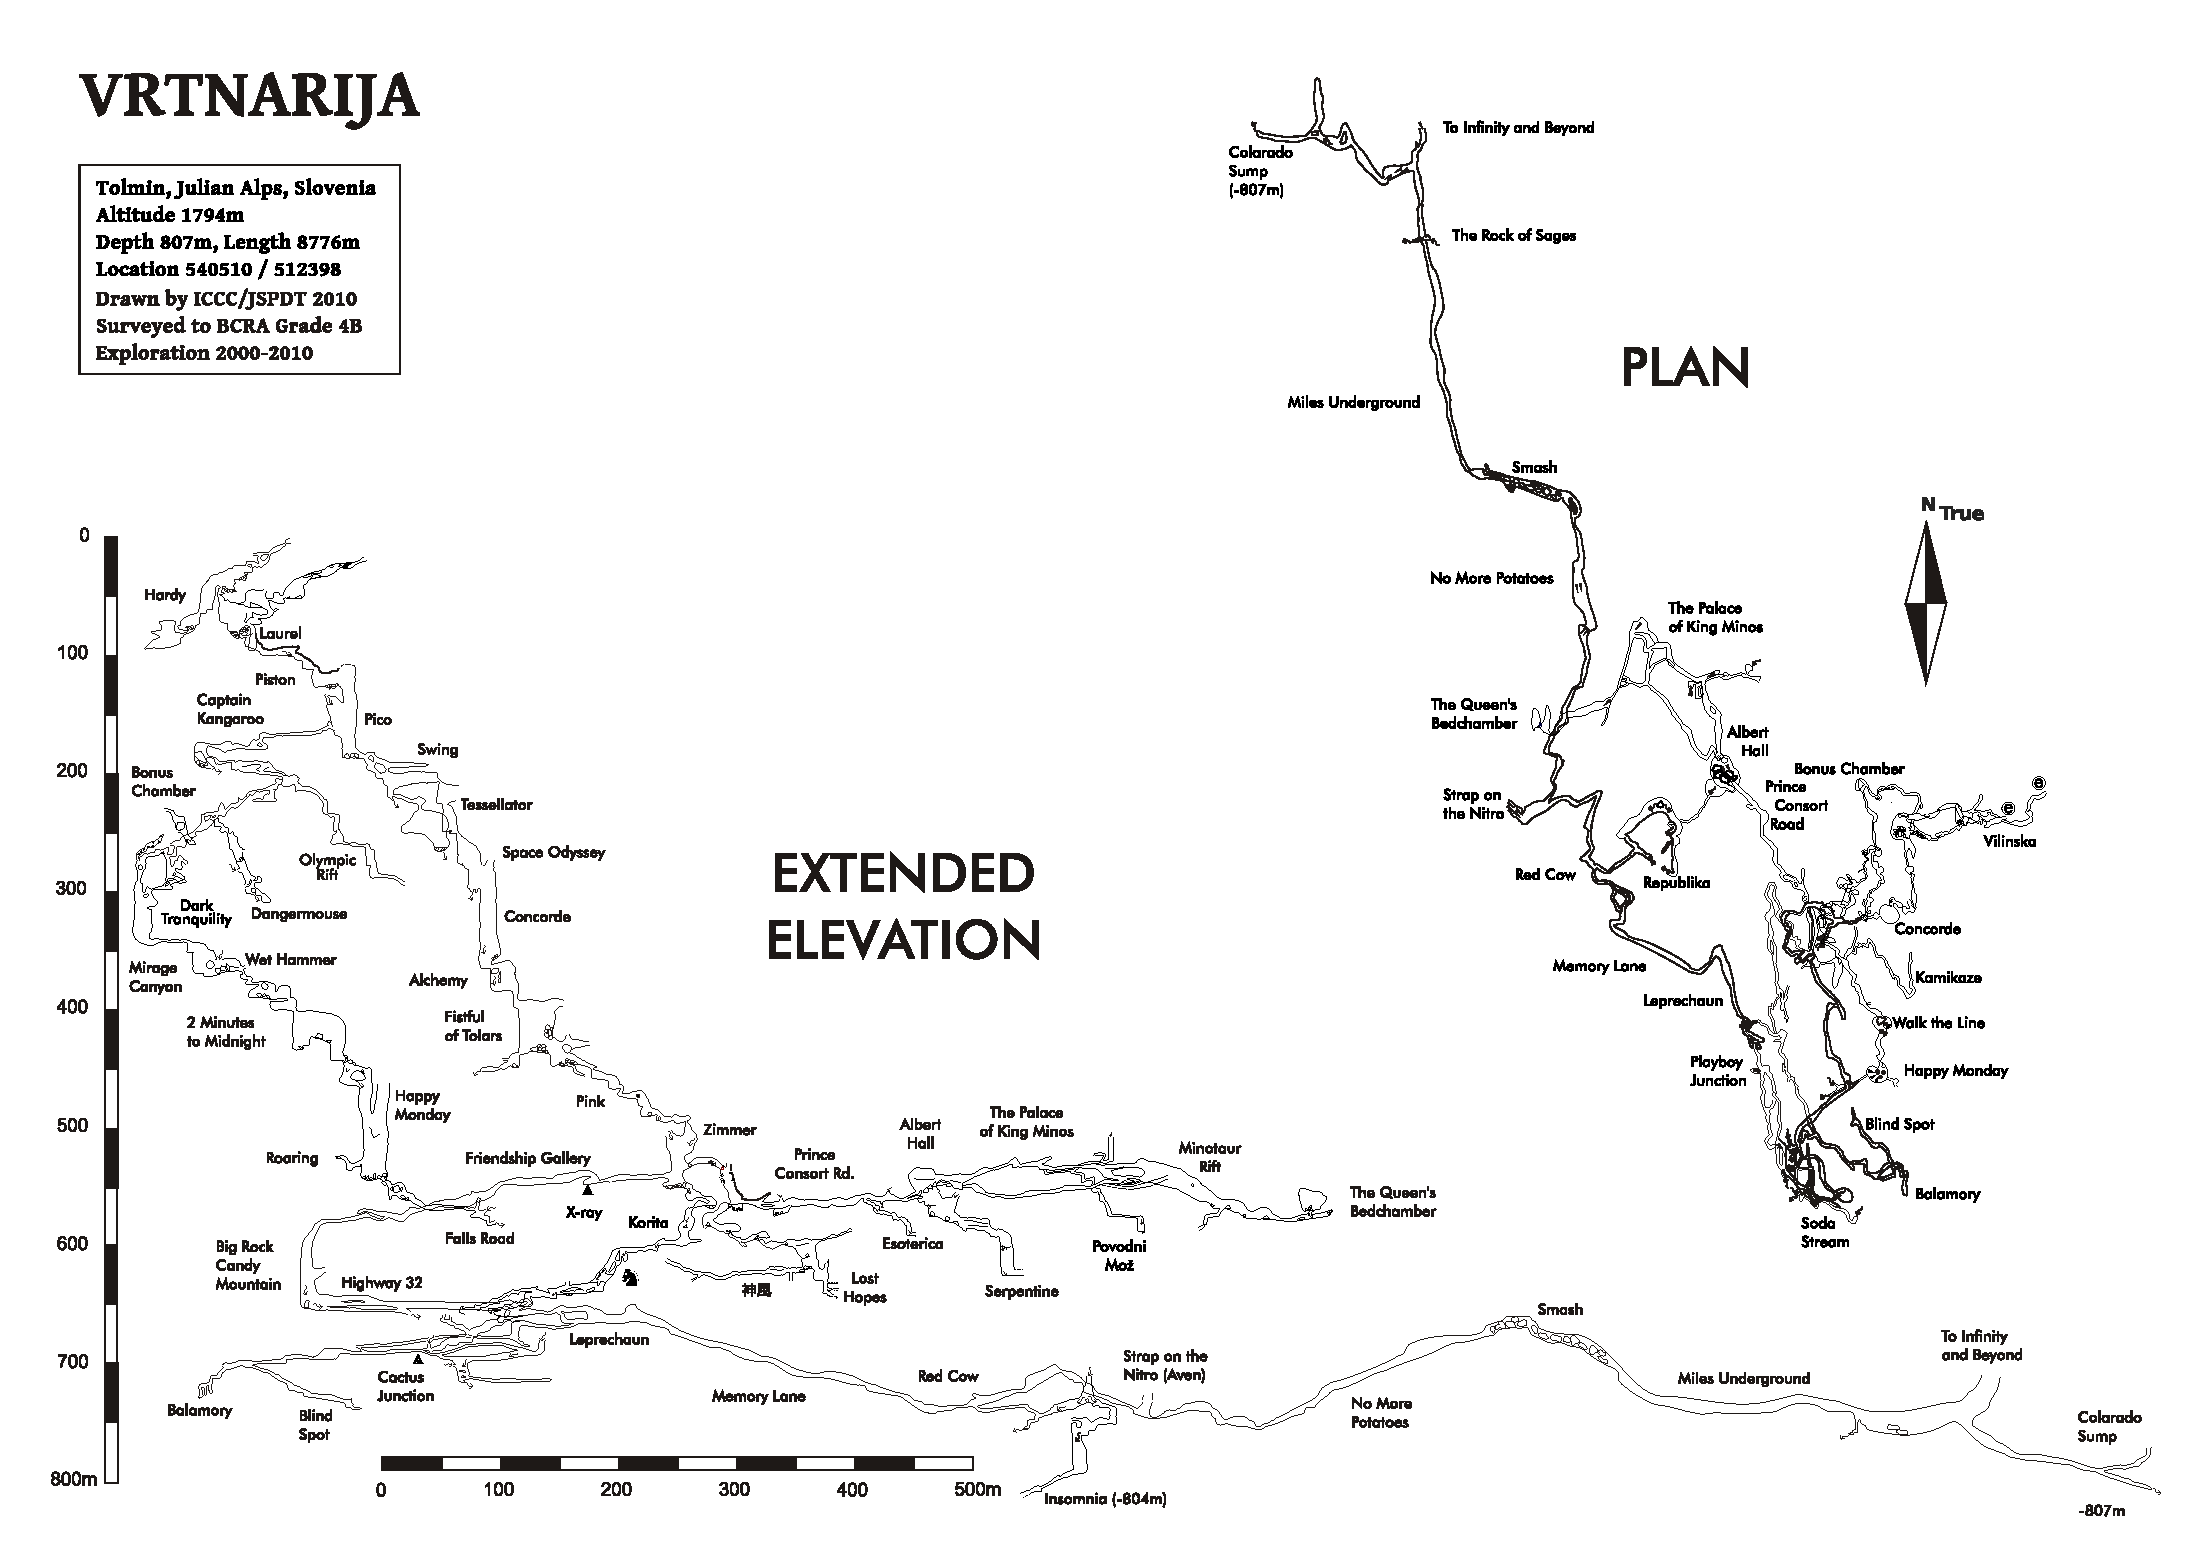
\includegraphics[width=\textheight, angle=90]{2010/survey/gw_2011-01-31.pdf}}
\caption[2010 Vrtnarija Survey]{2010 \passage{Vrtnarija} Survey}
\end{pagesurvey}


\begin{pagesurvey}
\centering
\frame{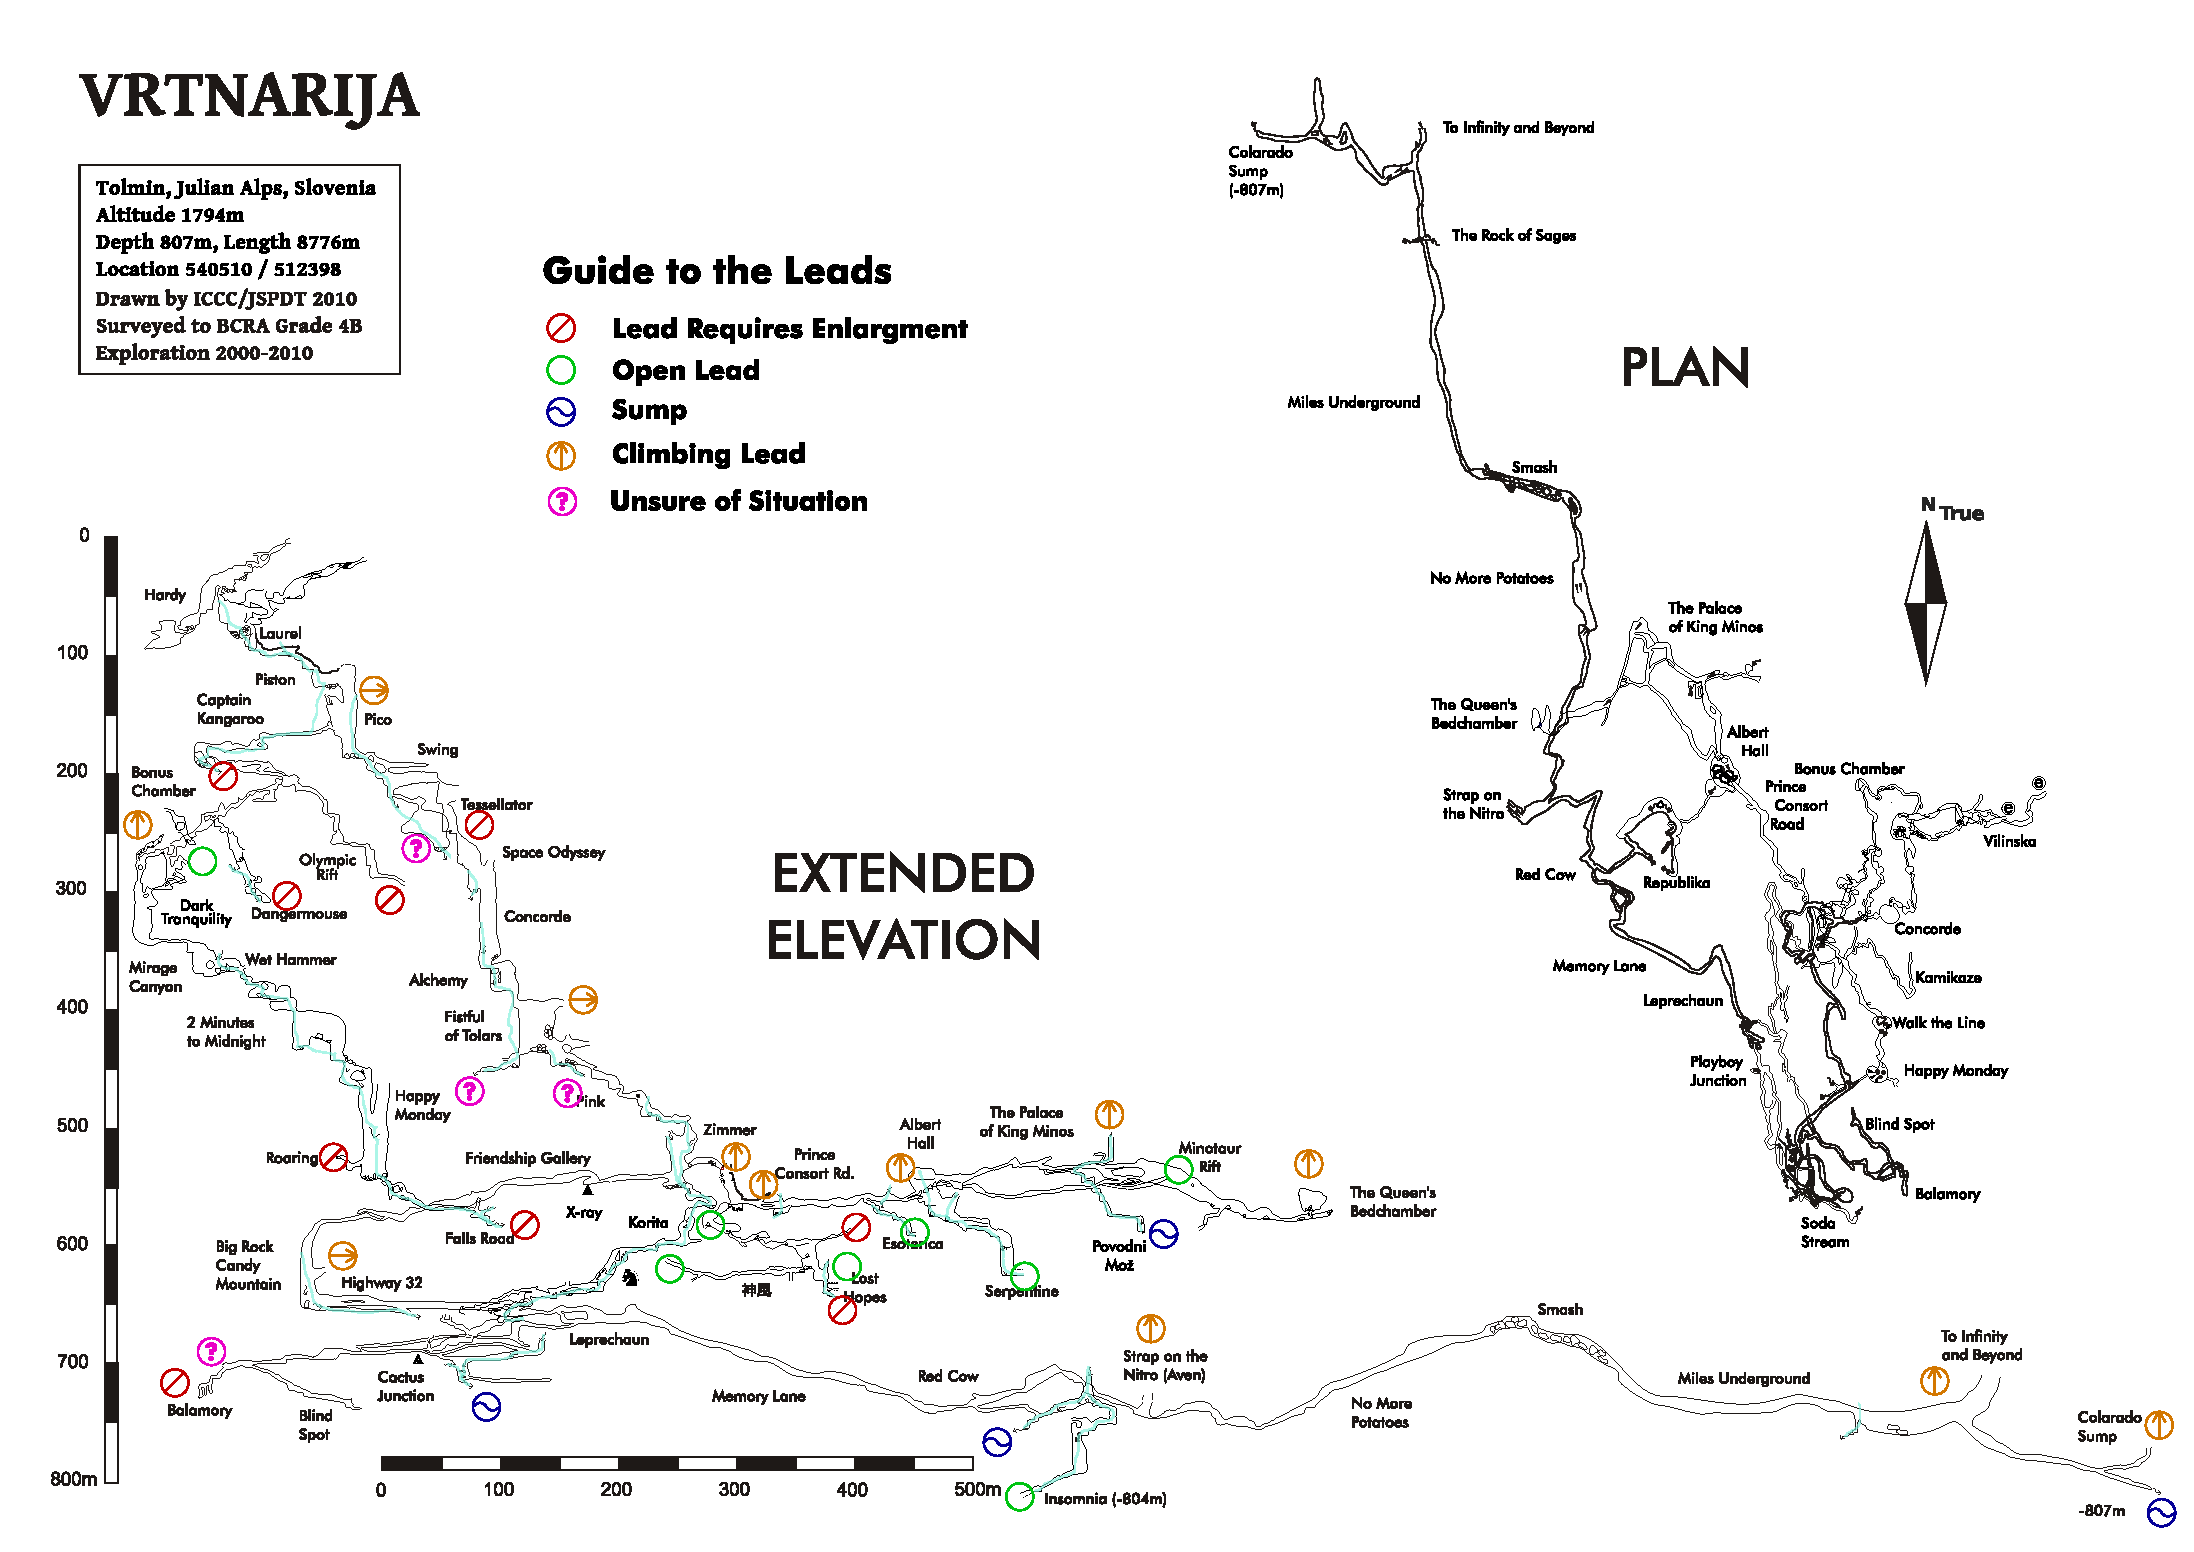
\includegraphics[width=\textheight, angle=90]{2010/survey/gw_2011-01-31-leads_water.pdf}}
\caption[2010 Vrtnarija Survey with Leads and Water Highlighted]{2010 \passage{Vrtnarija} Survey  with Leads and Water Highlighted}
\end{pagesurvey}